\documentclass[10pt, final, twoside]{article}

\usepackage[T2A]{fontenc}
\usepackage[utf8x]{inputenc}

\usepackage[russian, english]{babel}

\usepackage{float}
\usepackage[default]{lato}
\usepackage{textcomp}
\usepackage{amsmath, amssymb}
\usepackage{hyperref}
\usepackage[dvipsnames]{xcolor}
\usepackage[document]{ragged2e}
\usepackage[export]{adjustbox}
\usepackage{setspace}
\setstretch{1.5}

\usepackage{vmargin}
\setpapersize{A4}
\setmarginsrb{1cm}{1cm}{1cm}{1cm}{0pt}{0mm}{0pt}{13mm}

\usepackage{graphicx}

\renewcommand\arraystretch{1.8}
\newcommand{\No}{\textnumero}

\definecolor{darkgray2}{HTML}{434343}
\definecolor{darkgray4}{HTML}{cccccc}
\newcommand{\skill}[1]{\colorbox{darkgray4}{\textcolor{darkgray2}{#1}}}

\sloppy
\begin{document}
  \begin{minipage}{0.15\textwidth}\fbox{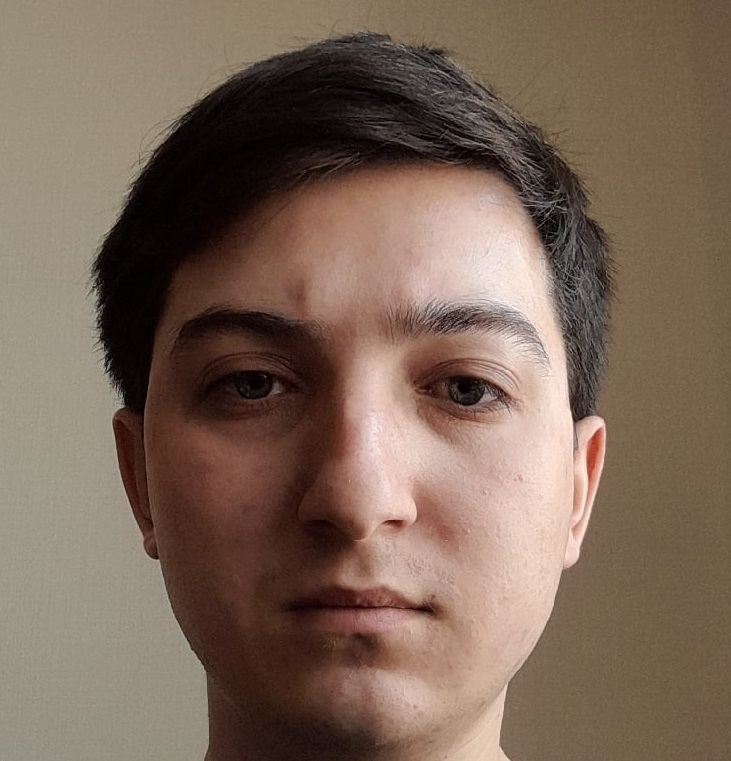
\includegraphics[width=\linewidth, right]{cv_photo.jpg}}\end{minipage}
  \begin{flushright}\section*{\textcolor{darkgray2}{Ханнанов Ленар Ильнурович}}\end{flushright}
  \vspace*{-5.5mm}
  \par\noindent\rule{\textwidth}{0.1pt}
  \textbf{Дата рождения:} 28 октября 2000.
  
  \textbf{Занятость:} проектная работа, стажировка, частичная занятость.
  
  \textbf{График работы:} удаленная работа, гибкий график, сменный график.

  \subsection*{\textcolor{darkgray2}{Контакты}}
  \vspace*{-5.5mm}
  \par\noindent\rule{\textwidth}{0.1pt}
  \begin{itemize}
    \item[\textcolor{MidnightBlue}{\textbullet}] \textcolor{MidnightBlue}{\underline{\url{https://t.me/come_ill_foo}}}
    \item[\textcolor{MidnightBlue}{\textbullet}] \href{mailto:khannanov2000@yandex.ru}{\textcolor{MidnightBlue}{\underline{khannanov2000@yandex.ru}}}
    \item[\textcolor{MidnightBlue}{\textbullet}] \href{tel:79279334902}{+7(927)933-49-02}
  \end{itemize}

  \begin{itemize}
    \item \textbf{195298}, Санкт-Петербург, м. Ладожская
  \end{itemize}

  
  \subsection*{\textcolor{darkgray2}{Опыт работы}}
  \vspace*{-5.5mm}
  \par\noindent\rule{\textwidth}{0.1pt}
  \begin{table}[H]
    \begin{tabular}{ll}
      08.2021--09.2021 & \textbf{RusEFI}\\
                       & \textbf{Программист}\\
                       & 1. Исправлял баги в приложении на Java+Swing\\
                       & 2. Осуществлял миграцию с системы сборки Apache Ant на Gradle 
    \end{tabular}
  \end{table}
  \begin{table}[H]
    \begin{tabular}{ll}
      02.2022--08.2022 & \textbf{ООО "Скайтек"}\\
                       & \textbf{Программист}\\
                       & 1. Проверял работу пропатченного ядра Linux (5.11, 5.17) на эмуляторе   Renode\\
                       & для микроконтроллеров на базе RISC-V архитектуры с MMU (BeagleV) и бе   (Kenryte K210)\\
                       & 2. Настраивал маршрутизатор iRZ R2 на общение по COM-порту    существующим бэкендом\\
                       & на Python (Flask)
    \end{tabular}
  \end{table}

  \subsection*{\textcolor{darkgray2}{Образование}}
  \vspace*{-5.5mm}
  \par\noindent\rule{\textwidth}{0.1pt}
  \begin{table}[H]
    \begin{tabular}{ll}
      2019--2023 & \textbf{НИУ ИТМО, Санкт-Петербург, 09.03.04, ПИИКТ, Системное Программное Обеспечение}
    \end{tabular}
  \end{table}

  \subsection*{\textcolor{darkgray2}{Ключевые навыки}}
  \vspace*{-5.5mm}
  \par\noindent\rule{\textwidth}{0.1pt}
    \skill{C/C++} \skill{Linux} \skill{Git} \skill{Python} \skill{PostgreSQL} \skill{Assembler} \skill{Java} \skill{Redis} \skill{Vue 3} \skill{Flask} \skill{Verilog HDL} \skill{Bash} \skill{GNU Make} \skill{Gradle} \skill{Binutils}

  \subsection*{\textcolor{darkgray2}{Знание языков}}
  \vspace*{-5.5mm}
  \par\noindent\rule{\textwidth}{0.1pt}
  \begin{itemize}
    \item Русский ~--- родной
    \item Английский ~--- B2 ~--- Средне-продвинутый
    \item Немецкий ~--- A1 ~--- начальный
  \end{itemize}

  \subsection*{\textcolor{darkgray2}{Онлайн-курсы}}
  \vspace*{-5.5mm}
  \par\noindent\rule{\textwidth}{0.1pt}
  \begin{table}[H]
    \begin{tabular}{ll}
      2020 & \textbf{Computer Science Center (CS Центр)}\\
           & Введение в архитектуру ЭВМ. Элементы операционных систем\\\hline
      2020 & \textbf{СКБ Контур}\\
           & Проектирование на C\#\\\hline
      2021 & \textbf{Университет ИТМО}\\
           & Встроенные системы\\\hline
      2022 & \textbf{Computer Science Center (CS Центр)}\\
           & Основы программирования для Linux\\\hline
      2022 & \textbf{Computer Science Center (CS Центр)}\\
           & Операционные системы\\\hline
    \end{tabular}
  \end{table}

  \subsection*{\textcolor{darkgray2}{О себе}}
  \vspace*{-5.5mm}
  \par\noindent\rule{\textwidth}{0.1pt}
  
Бакалавриат (4 курс). В свободное время люблю поигрывать в видеоигры.

Ниже расписал, чем увлекаюсь в профессиональной деятельности, включил все, что как-то смотрел, трогал в реальной жизни (это в основном про микроконтроллеры) и изучал в рамках университетской программы.

Сейчас пытаюсь освоить популярный язык для embedded и IoT -- Rust.
\end{document}
